\documentclass[runningheads]{llncs}

\usepackage[T1]{fontenc}
\usepackage{graphicx}
\usepackage{amsmath,amssymb}
\usepackage{booktabs}
\usepackage{array}
\usepackage{multirow}
\usepackage{makecell}
\usepackage{pifont}
\usepackage{algorithm}
\usepackage{algpseudocode}
\usepackage{xcolor}
\usepackage[hidelinks]{hyperref}
\usepackage{url}

% Compact lists / spacing helpers for 15-page LNCS budget
\usepackage{enumitem}
\setlist{itemsep=1pt,topsep=2pt,parsep=0pt}

% Float-packing: allow more of each page to be floats, less forced whitespace
\renewcommand{\topfraction}{0.92}
\renewcommand{\bottomfraction}{0.85}
\renewcommand{\textfraction}{0.06}
\renewcommand{\floatpagefraction}{0.82}
\setcounter{topnumber}{3}
\setcounter{totalnumber}{4}
\setlength{\textfloatsep}{9pt plus 2pt minus 2pt}
\setlength{\intextsep}{9pt plus 2pt minus 2pt}
\setlength{\abovecaptionskip}{4pt}
\setlength{\belowcaptionskip}{2pt}

% Custom macros
\newcommand{\silr}{\textsc{SiLR}}
\newcommand{\Phimeas}{\Phi}
\newcommand{\Cset}{\mathcal{C}}
\newcommand{\nfn}{n}
\newcommand{\Pfn}{P}
\newcommand{\psione}{\psi_1}
\newcommand{\psitwo}{\psi_2}
\newcommand{\psithree}{\psi_3}

\begin{document}

% Double-blind: anonymized author block
\title{\silr{}: Structured Recovery Admission for LLM Tool Proposals in Critical Infrastructure}
\titlerunning{Structured Recovery Admission for LLM Agents}

\author{Anonymous Author(s)}
\authorrunning{Anonymous}
\institute{Anonymous Institution \\ \email{anon@example.org}}

\maketitle

\begin{abstract}
Runtime enforcement keeps an AI-driven critical-infrastructure system inside its safe set; it does not say what to do once the system is \emph{already} in violation and must recover over multiple steps. We study this \emph{post-violation recovery admission} problem and frame it around \emph{admission semantics}---the criterion by which a runtime gate applies or rejects an LLM-proposed action. A terminal gate (admit only fully-recovered post-states) is safe but deadlocks multi-step recovery; the natural relaxation, a \emph{scalar admission gate} admitting any proposal whose aggregate violation penalty is non-increasing within a small slack, is structurally insufficient.

We identify the \emph{scalar projection trap}: in a ReAct-style control loop the verifier is not only a final filter but a search operator over the LLM's proposal stream. A scalar gate can then accept one early locally-improving proposal that commits the trajectory toward a residual plateau from which recovery may be unreachable. We propose \silr{}, a simulator-backed structured admission layer in which each LLM tool proposal is shadow-executed and admitted only when a product order over the branch-level violation state---overloaded-branch support and per-branch severity---is preserved. \silr{} emits graded \texttt{PASS}, \texttt{SAFE\_PROGRESS}, and \texttt{FAIL} verdicts.

On mined Gym-ANM scenarios (Qwen3-14B, $N{=}7$), structured graded admission recovers $\mathbf{21/21}$ multi-action episodes at zero residual penalty, where terminal admission deadlocks ($0/21$) and the best scalar slack reaches only $9/21$ (non-monotonic, with disjoint Wilson 95\% CIs); we make the gap precise as a representational impossibility. On the full $24$-scenario band structured admission recovers $117/120$, with scalar failures localizing to the geometry-poor operating points the trap predicts. The dichotomy holds across three model families and a second domain (CityLearn), demonstrating structural portability. Because admission grounds in deterministic simulation rather than the LLM's input channels, the trust boundary shifts from the LLM to the verifier; containment is thus \emph{architectural}: under a fixed compromised-LLM adversary a $75$-episode mini-suite yields $0/75$ attack-success, false-recovery, and material worsening. Finally, the same verifier reused as a GRPO process reward is internalized: the trained policy recovers without the gate and generalizes to held-out scenarios, with the product-order geometry the active ingredient.

\keywords{Runtime governance \and LLM agents \and Safety shielding \and Critical infrastructure \and Adversarial robustness.}
\end{abstract}

\section{Introduction}
\label{sec:intro}

Critical infrastructures---power dispatch, datacenter scheduling, financial settlement---are increasingly automated by tool-using large language model (LLM) agents~\cite{gridagent2025}, and a wave of runtime-enforcement systems (SARC~\cite{sarc2026}, AgentSpec~\cite{agentspec2026}, GuardAgent~\cite{guardagent2025}, ShieldAgent~\cite{shieldagent2025}, VeriGuard~\cite{veriguard2025}) makes them more governable. These systems share a rarely-stated assumption: the system starts \emph{inside} the safe set and the gate's job is to keep it there. But infrastructure under autonomous control will sometimes start \emph{outside} it---already in violation, needing a multi-step sequence to recover---and there the enforcement question inverts: the gate must decide whether an action that still leaves the system unsafe nonetheless makes admissible progress toward recovery. This \emph{post-violation recovery admission} problem is structurally different from prevention and largely unaddressed; runtime mediation intercepts unsafe actions yet rarely converts blocked ones into safe completion~\cite{verifiertax2026}. Enforcement is not recovery.

We frame the problem around \emph{admission semantics}: the formal criterion by which a runtime gate decides to apply or reject an LLM-proposed action. Our thesis is that this choice---not the gate's strictness---has first-order effects on whether multi-step recovery is possible. A terminal gate (admit only fully-recovered post-states) is safe but admits no intermediate step, deadlocking every multi-action episode on our mined Gym-ANM~\cite{henry2021gymanm} benchmark. The natural relaxation admits any proposal whose aggregate violation penalty is non-increasing within a small slack---a \emph{scalar admission gate}---and our central finding is that it is structurally insufficient, not for want of threshold tuning.

The reason is the \textbf{scalar projection trap}. In a ReAct loop a rejected proposal is followed by another at the same state, so \emph{the gate is not a filter but a search operator over the agent's proposal stream}; admitting on an aggregate score collapses the multi-component violation geometry and can commit the trajectory to a residual plateau from which recovery may be unreachable, whereas a gate that preserves the per-branch geometry declines the geometry-poor step and keeps the search alive. The gap is representational, which we make precise as a lower bound (Sec.~\ref{sec:method:trap}): structured admission recovers $\mathbf{21/21}$ multi-action episodes where the best scalar slack reaches $9/21$ and terminal $0/21$, with disjoint Wilson 95\% CIs.

\paragraph{Contributions.}
\begin{enumerate}
\item \textbf{The scalar projection trap.} We identify and characterize a failure mode of natural scalar recovery gates: viewed as a search operator over the ReAct proposal stream, a scalar gate can commit the trajectory to a residual plateau because aggregate penalty collapses the per-branch violation geometry the structured order retains (Sec.~\ref{sec:method:trap}). This reframes admission from a safety check into a trajectory-shaping mechanism.
\item \textbf{Structured recovery admission.} We propose \silr{}, a simulator-backed admission layer that shadow-executes each LLM tool proposal and admits it only when a product order over the branch-level violation state is preserved, emitting graded \texttt{PASS}/\texttt{SAFE\_PROGRESS}/\texttt{FAIL} verdicts (Sec.~\ref{sec:method}).
\item \textbf{Empirical validation with a falsification baseline, across families and a second domain.} Terminal admission deadlocks and a scalar threshold sweep cannot close the gap to structured admission; a plateau spectrum and an MPC feasibility check confirm the mechanism is gate-induced (Sec.~\ref{sec:eval:rq1}--\ref{sec:eval:rq3}). The terminal-versus-structured dichotomy holds across three independent model families and reproduces in a second domain (CityLearn): structured admission lets compact open-weight models perform the multi-step recovery that binary and scalar gates cannot (Sec.~\ref{sec:eval:rq5}).
\item \textbf{Trust-boundary containment.} Because admission grounds in deterministic simulation rather than the LLM's input channels, containment is \emph{architectural}, not statistical: a security mini-suite under compromised prompts, observations, and stall instructions yields zero attack-induced worsening or false recovery (Sec.~\ref{sec:eval:rq4}).
\end{enumerate}

\paragraph{Regime and deployment model.}
Our target regime is multi-component concurrent violation---where a scalar penalty aggregates a multi-component severity vector and the projection trap arises---instantiated by Gym-ANM's branch-loading family. \silr{} is an advisory-layer gate at the medium-horizon dispatch loop, where LLM latency is compatible with the pre-dispatch power-flow study. We evaluate this regime in depth and test generalization across three model families and a second domain (CityLearn).

\section{Related Work}
\label{sec:related}

\paragraph{Shielding and recoverability-set safe RL.}
Shielding~\cite{alshiekh2018safe} synthesizes a finite-state shield from a temporal-logic specification that intercepts policy outputs at runtime; Model-Predictive Shielding~\cite{bastani2019mps}, Recovery RL~\cite{thananjeyan2021recovery}, and RL power-grid shielding~\cite{hrlshield2026} relax binary terminal gates by admitting recoverability-set states or screening actions with forward simulation. All assume a fixed action space and require either a backup/recovery policy or a dynamics-model lookahead. \silr{} instead shields \emph{black-box LLM tool-call dispatch} with neither: proposals are admitted by single-step shadow simulation under a product order on the branch-level violation state, at constant per-step cost. Where these lineages apply a fixed admissibility filter to a known action model, \silr{} makes admission itself the design variable---a graded predicate over violation geometry.

\paragraph{Runtime guards for LLM agents.}
Recent work adds runtime enforcement to tool-using LLM agents through architectural gates, guard agents, or rule languages: SARC's Pre-Action Gate~\cite{sarc2026} (the closest binary baseline, admitting a tool call only when a hand-written predicate holds), AgentSpec's runtime-enforcement DSL~\cite{agentspec2026}, GuardAgent~\cite{guardagent2025} and ShieldAgent~\cite{shieldagent2025} (compiling guard policies), and VeriGuard~\cite{veriguard2025} (verified code generation plus monitoring). These make LLM agents more governable but do not target post-violation recovery admission: a terminal predicate (as a SARC-style Pre-Action Gate instantiates) preserves safety but deadlocks multi-step recovery (Sec.~\ref{sec:eval:rq1}).

\paragraph{LLM agents for power-grid control.}
Grid-Agent~\cite{gridagent2025} is the closest same-domain near-neighbor: it couples LLM agents with sandboxed power-flow validation, rollback of negative actions, and monotonic-progress behavior for power-grid control. The mechanisms differ in kind: Grid-Agent's check is a \emph{post-hoc} rollback that reverts an action unless the violation set is resolved without introducing new violations---a support-level criterion with no per-branch severity guard---whereas \silr{}'s product order is a \emph{pre-action} admission predicate that never applies a geometry-poor step and emits graded verdicts reusable as a training signal.

\paragraph{Multi-objective optimization and scalarization.}
Scalarization trade-offs are classically studied as a \emph{static} representational question---e.g., linear scalarization cannot reach non-convex Pareto regions~\cite{miettinen1999nonlinear}. The scalar projection trap (Sec.~\ref{sec:method:trap}) is a \emph{behavioral} phenomenon of the runtime gate: in a ReAct loop the gate is a commitment operator, so an admitted aggregate-improving step restarts the per-step search from a plateau state---a failure of the gate's trajectory dynamics, not merely of an aggregate's expressiveness.

\paragraph{Adversarial LLM defenses.}
Prompt injection~\cite{greshake2023injection} is a documented attack vector; prior defenses sanitize inputs or outputs. \silr{} adopts a third stance: the LLM \emph{may} be compromised, and safety is enforced after the proposal by shadow-executing it on the simulator, shifting the trust boundary from the LLM to the verifier and simulator.

\paragraph{Positioning.}
Table~\ref{tab:related} places \silr{} against the closest systems along four axes: \emph{graded} admission (beyond binary accept/reject), \emph{retained multi-component violation geometry} (vs.\ a scalar aggregate), \emph{black-box LLM tool proposals} (no fixed action space), and \emph{neither a backup/recovery policy nor a multi-step dynamics lookahead}. \silr{} is the only point meeting all four---this combination is the contribution.

\begin{table}[tb]
\centering
\caption{Positioning of \silr{} against the closest runtime-safety systems. ``Geometry'': retains the (support, severity) violation state vs.\ a scalar aggregate; ``No lookahead/backup'': single-step shadow only, no recovery policy or dynamics rollout.}
\label{tab:related}
\footnotesize
\setlength{\tabcolsep}{4pt}
\begin{tabular*}{\textwidth}{@{\extracolsep{\fill}}lcccc}
\toprule
System & Graded & Geometry & \makecell{Black-box\\LLM} & \makecell{No lookahead/\\backup} \\
\midrule
SARC Pre-Action Gate~\cite{sarc2026}        & \ding{55} & \ding{55} & \ding{51} & \ding{51} \\
AgentSpec DSL~\cite{agentspec2026}          & \ding{55} & \ding{55} & \ding{51} & \ding{51} \\
GuardAgent/ShieldAgent~\cite{guardagent2025,shieldagent2025} & \ding{55} & \ding{55} & \ding{51} & \ding{51} \\
Grid-Agent~\cite{gridagent2025}             & \ding{55} & \ding{55}$^\dagger$ & \ding{51} & \ding{55}$^\ddagger$ \\
MPS / Recovery RL~\cite{bastani2019mps,thananjeyan2021recovery} & \ding{55} & \ding{55} & \ding{55} & \ding{55} \\
\silr{} (ours)                              & \ding{51} & \ding{51} & \ding{51} & \ding{51} \\
\bottomrule
\end{tabular*}\\[2pt]
{\footnotesize $^\dagger$support-level violation validation, no per-branch severity guard; $^\ddagger$applies then reverts (post-hoc rollback).}
\end{table}

\section{Trust Boundary and Adversary Model}
\label{sec:threat}

\silr{} relocates the trust boundary from the LLM to the shadow simulator: no admission verdict depends on the LLM's reasoning, only on the simulator's deterministic response. We fix the adversary here---before the mechanism (Sec.~\ref{sec:method})---since it shapes what the gate must defend. The LLM is untrusted; the simulator, verifier, checkers, and tool layer are trusted.

\paragraph{Adversary capability.}
We adopt the compromised-prompt and compromised-observation capability class (the union of the SARC~\cite{sarc2026} and VeriGuard~\cite{veriguard2025} threat models). An attacker may (C1)~rewrite the system prompt, including operator-directive impersonation; (C2)~splice attacker-controlled text into every observation; and (C3)~persist both rewrites for the whole episode without reacting to LLM behavior (worst case for the defender). The attacker may \emph{not} modify the verifier, checkers, manager, simulator, or tool-layer validators, bypass \texttt{apply\_action}, or read the verifier's shadow state. Network, side-channel, supply-chain, and adaptive adversaries (tuning injections against observed verdicts) are out of scope (Sec.~\ref{sec:discussion}).

\paragraph{Failure semantics.}
Two primary outcomes and one derived. \emph{Material worsening}: the trajectory ends with strictly higher final penalty than the no-intervention default---worse than doing nothing. \emph{False recovery}: the trajectory reports terminal recovery while the live simulator state still contains violations. \emph{Attack success} (derived): the union of the two---any safety-relevant outcome the benign trajectory would have avoided. A recovery-rate drop without any of these is a liveness limitation, not a safety failure.

\paragraph{Instantiated attacks.}
We implement four attack families (detailed in Sec.~\ref{sec:eval:rq4}): \emph{prompt injection} (C1, a high-priority override pushing an aggressive fixed setpoint), \emph{observation poisoning} (C2, a fabricated ``all readings nominal'' stanza contradicting the violation list the verifier re-derives), \emph{stall} (C1, near-no-op setpoints that stay admissible while never recovering; a ``stall-RAG'' variant instructs the same), and \emph{magnitude redistribution} (C1/C2, driving a single retained branch toward failure while holding the overloaded-branch set and aggregate penalty within nominal bounds, masking per-branch overload behind nominal aggregate- and support-level readings).
\section{Method: Structured Recovery Admission}
\label{sec:method}

\subsection{Setting: Post-Violation Recovery in a ReAct Loop}
\label{sec:method:setting}

We consider an LLM tool-calling agent that controls a critical-infrastructure simulator $M$ through a ReAct loop. At each control step $t=1,\ldots,C_{\text{step}}$, the agent observes $\mathit{obs}_t$, proposes a tool call $a_t$, and the proposal is mediated by a runtime verifier before it is applied. If the verifier rejects $a_t$, the agent generates another proposal within the same step, up to a per-step proposal budget $C_{\text{prop}}$. \emph{Post-violation} initial conditions mean $M$ starts in a state $s_0$ with one or more active constraint violations; the goal is to drive $M$ to a violation-free state through a sequence of admitted tool calls.

Two consequences make admission semantics the central object: a \emph{terminal} gate (admit only fully-recovered post-states) stalls multi-action recovery; and since a rejected proposal triggers another within the step, the gate is a \emph{search operator} over the proposal stream, not a fixed filter---which nonterminal states it admits shapes the trajectories explored.

\subsection{Shadow-Execution Verifier}
\label{sec:method:shadow}

For each candidate $a_t$, the verifier evaluates a deterministic shadow state
\begin{equation}
\hat{s}_{t+1} \;=\; \mathrm{shadow}(s_t,a_t)\;=\;\mathrm{solve}\bigl(\mathrm{apply}(\mathrm{copy}(s_t),\,a_t)\bigr),
\end{equation}
where $\mathrm{solve}(\cdot)$ is the domain's steady-state solver (Newton--Raphson power flow for Gym-ANM~\cite{henry2021gymanm}), run on a deep copy of $M$ so rejected proposals leave the live system untouched. The verifier emits a verdict from $\{\texttt{PASS}, \texttt{SAFE\_PROGRESS}, \texttt{FAIL}, \texttt{ERROR}\}$ and applies the admitted ($\texttt{PASS}$/$\texttt{SAFE\_PROGRESS}$) action. The trust boundary is explicit: the LLM may be compromised, but the verdict depends on the simulator's deterministic response to the action, not on the LLM's reasoning.

\subsection{Branch-Level Violation State and the Verdict Ladder}
\label{sec:method:state}

Let $V_k:S\to\{\text{pass},\text{fail}\}$ be the $k$-th constraint checker emitting a violation multiset $\mathbf{v}_k(s)$. We focus on the active violation family in our benchmark, branch loading, whose violation is naturally indexed by overloaded branch. Define the branch-level violation state
\begin{equation}
\Phi(s) \;=\; \bigl(S(s),\,\sigma(s)\bigr),
\quad
S(s)\subseteq\mathcal{B},
\quad
\sigma(s)\in\mathbb{R}_{\ge 0}^{|\mathcal{B}|},
\label{eq:phi}
\end{equation}
where $\mathcal{B}$ is the set of branches, $S(s)$ is the support set of currently overloaded branches, and $\sigma(s)$ is the per-branch severity vector ($\sigma_i(s)\,{>}\,0$ iff $i\in S(s)$). The fully-recovered state satisfies $S(s)=\emptyset$ (equivalently $\sigma(s)=\mathbf{0}$). The count is $n(s)=|S(s)|$ and the aggregate penalty is $P(s)=\sum_i\sigma_i(s)$. We equip the state space with the product partial order
\begin{equation}
\Phi(s)\preceq\Phi(s')
\;\iff\;
S(s)\subseteq S(s')
\;\wedge\;
\sigma(s)\le\sigma(s')\text{ componentwise},
\end{equation}
where support inclusion already subsumes count non-increase, since $n(s)=|S(s)|$ and $S(s)\subseteq S(s')\Rightarrow n(s)\le n(s')$; we therefore order directly on support and per-branch severity. This order is precisely \emph{Pareto dominance} on the vector-valued violation state $(S,\sigma)$: admitting only $\Phi$-non-increasing steps is a vector-valued (Pareto-improvement) admission rule, of which a scalar penalty gate is the one-dimensional projection. We call $\hat{s}_{t+1}$ \emph{admissible} from $s_t$ if $\Phi(\hat{s}_{t+1})\preceq\Phi(s_t)$, relaxed in practice to the $\varepsilon$-dominance order $\preceq_{\alpha,\varepsilon}$ of Sec.~\ref{sec:method:predicates}. The verdict ladder is then
\texttt{PASS} if $S(\hat{s}_{t+1})=\emptyset$ (terminal recovery); \texttt{SAFE\_PROGRESS} if $\Phi(\hat{s}_{t+1})\preceq\Phi(s_t)$ but $S(\hat{s}_{t+1})\ne\emptyset$ (admissible nonterminal progress); \texttt{FAIL} otherwise. Our benchmark exercises one dominant violation family (branch loading) over multiple concurrent overloaded components, so the order acts on the $(S,\sigma)$ geometry within that family. Concurrent multi-family violations, and strongly-coupled regimes where recovery must transit a state that transiently overloads a clean branch (a non-monotone support path), are out of scope (Sec.~\ref{sec:discussion}).

\subsection{The Scalar Projection Trap}
\label{sec:method:trap}

A natural simpler design would replace the structured product order with a \emph{scalar admission gate}: admit $\hat{s}_{t+1}$ whenever the aggregate penalty $P(\hat{s}_{t+1})$ is non-increasing or within a small slack of $P(s_t)$. We now identify why this natural relaxation is structurally insufficient.

\paragraph{A representational lower bound.}
Any scalar surrogate projects the vector state $\Phi(s)=(S(s),\sigma(s))$ onto $\mathbb{R}_{\ge 0}$; the aggregate penalty $P(s)=\sum_i\sigma_i(s)$ is one such surrogate. Projecting a partial order with antichains onto a total order necessarily makes some incomparable states comparable:
\begin{proposition}[Scalarization gap]
\label{prop:gap}
No scalar surrogate is sound for $\preceq$: for any $f:(S,\sigma)\to\mathbb{R}_{\ge 0}$, a gate that admits whenever $f$ is non-increasing accepts, on some $\preceq$-antichain pair, a step that introduces or relocates a violation.
\end{proposition}
\begin{proof}
Take $\Phi(s)=(\{A\},\,2\delta\,e_A)$ and $\Phi(s')=(\{A,B\},\,0.9\delta(e_A{+}e_B))$ for any $\delta>0$; these are $\preceq$-incomparable, since $S(s')\not\subseteq S(s)$ while $\sigma_A(s)=2\delta>0.9\delta=\sigma_A(s')$. As $\mathbb{R}$ is totally ordered, $f$ ranks the pair, so the gate admits one of $s\!\to\!s'$ or $s'\!\to\!s$: the former adds branch $B$, the latter drives $\sigma_A$ from $0.9\delta$ to $2\delta$. Either step is non-improving under $\preceq$. The aggregate $P=\sum_i\sigma_i$ is the special case $P(s')=1.8\delta<2\delta=P(s)$. \qed
\end{proof}
The gap is intrinsic to projecting a partial order with antichains onto a total order, independent of the surrogate or threshold: relaxing the test to $f(\hat{s}_{t+1})\le(1{+}\eta)f(s_t)$ only enlarges the admissible set, never removing the collapse. \silr{} avoids the gap by admitting on $\preceq$ directly.

\paragraph{Mechanism: the gate as a commitment operator.}
This representational gap becomes a \emph{behavioral} failure through the search loop. A rejected proposal causes the agent to regenerate at the same $s_t$, so a scalar gate that admits the \emph{first} $P$-improving proposal ends the per-step search and commits the trajectory to $\hat{s}_{\text{bad}}$, from which further descent to $P=0$ may be infeasible---a residual plateau; a structured gate rejects the same geometry-poor proposal and keeps the search active. We call this the \textbf{scalar projection trap}: a runtime-gate manifestation of the classical scalarization gap~\cite{miettinen1999nonlinear}, made behavioral by the gate's per-step commitment. Scalar slack helps only where scalar descent and Pareto-admissibility coincide (Sec.~\ref{sec:eval:rq3}); no scalar projection is a \emph{general} recovery-admission semantics.

\subsection{Predicates and Apply-Gate}
\label{sec:method:predicates}

The implemented apply-gate is a conjunction of three predicates, evaluated on the shadow:
\begin{align}
\psione(a_t)\;&:\;\mathrm{tool}(a_t)\in\mathcal{A}_{\text{allowed}}\;\wedge\;\forall p\in\mathrm{params}(a_t):\mathrm{finite}(p)\wedge p\in[p_{\min},p_{\max}], \\
\psitwo(s_t,\hat{s}_{t+1})\;&:\;S(\hat{s}_{t+1})\subseteq S(s_t)\quad(\text{which implies }n(\hat{s}_{t+1})\le n(s_t)), \\
\psithree(s_t,\hat{s}_{t+1})\;&:\;\sigma_i(\hat{s}_{t+1})\le\max\bigl(\alpha\sigma_i(s_t),\,\sigma_i(s_t)+\varepsilon\bigr)\text{ for all }i\in S(s_t),
\end{align}
with $\alpha{=}1.05$, $\varepsilon{=}10^{-3}$. Together $\psitwo\wedge\psithree$ is the computable test for the relaxed order
\begin{equation}
\Phi(\hat{s})\preceq_{\alpha,\varepsilon}\Phi(s)\;\iff\;S(\hat{s})\subseteq S(s)\;\wedge\;\sigma_i(\hat{s})\le\max\bigl(\alpha\sigma_i(s),\,\sigma_i(s)+\varepsilon\bigr)\;\forall i,
\end{equation}
a per-branch \emph{$\varepsilon$-dominance}-style relaxation (in the sense of~\cite{laumanns2002}, applied here as an admission predicate rather than an archive criterion) that recovers exact Pareto dominance $\preceq$ as $\alpha\to1,\varepsilon\to0$. The two thresholds carry a principled reading: $\alpha$ absorbs the finite resolution of the agent's discrete action space and $\varepsilon$ numerical precision, the solver itself being deterministic to machine precision. This yields the gate's containment guarantee:
\begin{proposition}[Admission invariant]
\label{prop:inv}
Under shadow fidelity (the live system reproduces the shadow post-state, exact in our deterministic simulators), every admitted trajectory satisfies $S(s_t)\subseteq S(s_0)$ for all $t$, independently of LLM behavior; per-branch severity obeys $\sigma_i(s_t)\le\alpha^{t}\sigma_i(s_0)+\varepsilon\tfrac{\alpha^{t}-1}{\alpha-1}$.
\end{proposition}
\noindent(Induction on $t$: $\psitwo$ gives $S(s_{t+1})\subseteq S(s_t)$; $\psithree$ gives $\sigma_i(s_{t+1})\le\alpha\sigma_i(s_t)+\varepsilon$, unrolled; the bound reads $\sigma_i(s_0)+t\varepsilon$ at $\alpha{=}1$.) The support invariant is $\alpha$-free and holds for \emph{any} gated policy, including a compromised LLM---the containment guarantee a runtime shield should make. The severity term is a worst-case per-step drift envelope, not a descent guarantee: convergence to $S=\emptyset$ depends on proposal quality (Sec.~\ref{sec:discussion}). The action is applied iff $\psione\wedge\psitwo\wedge\psithree$; this realizes the verdict ladder of Sec.~\ref{sec:method:state} (with \texttt{ERROR} when $\psione$ fails on an invalid proposal).

We compare four runtime policies in Sec.~\ref{sec:eval}: \texttt{OFF} (no gate), \texttt{terminal} (admit only when $S(\hat{s}_{t+1})=\emptyset$), \texttt{progress} ($\psione\wedge\psitwo$), \texttt{progress\_mag} ($\psione\wedge\psitwo\wedge\psithree$; the structured admission gate, in which $\psitwo$ enforces the support containment recovery rides on and $\psithree$ adds a per-branch severity guard as defense-in-depth). A separate \texttt{scalar\_progress} policy substitutes a scalar threshold for $\psitwo\wedge\psithree$ as a falsification baseline, thresholding the domain-native penalty $P$---a monotone aggregate of per-branch severity, hence an instance of the surrogate $f$ in Prop.~\ref{prop:gap}---at $P(\hat{s}_{t+1})\le(1{+}\eta)P(s_t)$, $\eta\in\{0,0.05,0.10,0.20\}$. It emits the same verdict ladder, so the structured and scalar gates are directly comparable on which nonterminal states they admit. \silr{}'s design point---graded, geometry-preserving, black-box, and lookahead-free---is positioned against prior systems in Table~\ref{tab:related}.

\section{Evaluation}
\label{sec:eval}

The evaluation is a progressive falsification of existing gate designs (RQ1--RQ3), followed by validation of the structured gate's orthogonal properties---containment under attack (RQ4) and generalization (RQ5). \textbf{RQ1}: does a binary terminal gate deadlock multi-step post-violation recovery? \textbf{RQ2}: does scalar admission, swept up to $20\%$ slack, close the gap to structured admission? \textbf{RQ3}: does the predicted projection-trap plateau signature appear, and is it gate-induced rather than reflecting an unrecoverable underlying state? \textbf{RQ4}: under LLM-side compromise (prompt injection, observation poisoning, stall, and magnitude redistribution), does the verifier prevent system worsening and false recovery? \textbf{RQ5}: does the terminal-versus-structured dichotomy generalize across model families and a second domain?

\subsection{Setup}
\label{sec:eval:setup}

We use Gym-ANM ANM6-Easy~\cite{henry2021gymanm} as the critical-infrastructure simulator, integrated as a \silr{} domain with a deep-copy shadow manager and a Newton--Raphson power-flow solver that is bit-exact across repeated solves ($\sigma{=}0$ over $100$ trials). The LLM is Qwen3-14B~\cite{qwen3} served via vLLM at temperature $0$. Each ReAct episode runs with $C_{\text{step}}{=}8$ control steps and $C_{\text{prop}}{=}3$ per-step proposals.

\paragraph{Scenarios.}
We mine a 600-scenario pool by gridded perturbation of load/generation multipliers, source seed, and storage SoC, classified by recoverability (\emph{single-action} 153, \emph{multi-action} 24, \emph{MPC-residual} 252, trivial 171). The multi-action band---$8$ operating points $\times\,3$ storage-SoC perturbations---is our benchmark; each scenario is MPC-recoverable (gym-anm \texttt{MPCAgentConstant} oracle), so the comparison is well-posed. The matched deep contrast (RQ1--RQ3) uses three operating points at $N{=}7$, denoted \texttt{multi\_1}--\texttt{multi\_3} (seeds $1003$--$1009$, $21$ episodes each, $C_{\text{step}}{=}8$); to rule out scenario selection we additionally evaluate \emph{all $24$} at $N{=}5$. Generalization and security suites use $N{=}5$.

\paragraph{Policies.}
\texttt{OFF} (no verifier; every proposal applied), \texttt{terminal} (terminal predicate: admit iff $S(\hat{s}_{t+1})=\emptyset$), \texttt{progress} ($\psione\wedge\psitwo$), \texttt{progress\_mag} ($\psione\wedge\psitwo\wedge\psithree$; the structured admission gate). For the scalar falsifier we add \texttt{scalar\_progress}$_\eta$, admitting iff $P(\hat{s}_{t+1})\le(1{+}\eta)P(s_t)$ with $\eta\in\{0,0.05,0.10,0.20\}$.

\subsection{RQ1: Binary Terminal Admission Deadlocks Multi-Step Recovery}
\label{sec:eval:rq1}

Table~\ref{tab:rq1} reports the headline result at \emph{matched} $N{=}7$ under $C_{\text{step}}{=}8$. Terminal recovers $0/21$ (reject/prop $1.000$): it rejects every intermediate proposal because $S(\hat{s}_{t+1})\ne\emptyset$ at every proposed step, regardless of search depth. Structured admission recovers $\mathbf{21/21}$ (CI $[0.85, 1.00]$, residual $0.000$), while the scalar sweep peak ($9/21$) has a CI disjoint from it---the scalar gap is not sampling noise.

\begin{table}[tb]
\centering
\caption{RQ1: mined multi-action recovery at matched $N{=}7$ ($21$ episodes/policy, $C_{\text{step}}{=}8$). Scalar row = sweep peak ($\eta{=}0.05$); Wilson 95\% CI. Material worsening is $0/21$ for every gated policy; ungated \texttt{OFF} worsens $12/21$.}
\label{tab:rq1}
\footnotesize
\begin{tabular*}{\textwidth}{@{\extracolsep{\fill}}lcccc}
\toprule
Policy & Recovery & 95\% CI & \makecell{Final pen.\\(mean)} & \makecell{Reject /\\prop.} \\
\midrule
\texttt{OFF} (no gate)                      & $1/21$   & $[0.01,0.23]$ & $15.594$ & $0.000$ \\
\texttt{terminal}                           & $0/21$   & $[0.00,0.15]$ & $12.451$ & $1.000$ \\
\texttt{scalar\_progress} (sweep peak)      & $9/21$   & $[0.24,0.63]$ & $4.950$  & $0.408$ \\
\texttt{progress}                           & $20/21$  & $[0.77,0.99]$ & $0.195$  & $0.336$ \\
\texttt{progress\_mag}                      & $\mathbf{21/21}$ & $\mathbf{[0.85,1.00]}$ & $\mathbf{0.000}$ & $0.316$ \\
\bottomrule
\end{tabular*}
\end{table}

The terminal deadlock is structural---the gate refuses every intermediate proposal regardless of search depth---and the lift over the scalar peak ($9/21$) is structural too: support admission alone closes most of it (RQ2).

\subsection{RQ2: Scalar Admission Is Insufficient---A Threshold Sweep Falsifier}
\label{sec:eval:rq2}

If the binary terminal gate fails only because it is too strict, the natural fix is to admit any proposal whose aggregate penalty $P$ is non-increasing or within a small slack of $P(s_t)$. We test this directly with the \texttt{scalar\_progress} family, sweeping the relative slack $\eta$ from strict ($0$) to $20\%$ at matched $N{=}7$ ($21$ episodes/setting, $C_{\text{step}}{=}8$).

Relaxing the threshold neither closes the gap nor improves monotonically: across $\eta\in\{0,0.05,0.10,0.20\}$ recovery is $5/21$, $9/21$, $7/21$, $7/21$, with mean final penalties $4.7/5.0/4.2/2.9$ (default $12.451$) and Wilson 95\% CIs in $[0.11,0.63]$, all disjoint from structured admission's $21/21$ at $[0.85,1.00]$. The non-monotonicity is itself a trap signature: the $\eta{=}0.05\!\to\!0.10$ drop comes entirely from \texttt{multi\_1} ($1\!\to\!0$) and \texttt{multi\_3} ($2\!\to\!0$), while \texttt{multi\_2} rises monotonically to $7/7$. A trace shows the mechanism: on \texttt{multi\_3} (seed $1004$) $\eta{=}0.05$ rejects a step's first two proposals and admits a third, geometry-preserving one to recovery, whereas $\eta{=}0.10$ admits that first proposal and commits to a residual plateau ($P{=}10.86$)---wider slack recovers \emph{less} because admission is a commitment operator (Sec.~\ref{sec:method:trap}). A gate whose recovery rose monotonically in slack would contradict the trap; the non-monotonicity is direct evidence for it.

\paragraph{Structure, not magnitude, drives recovery.}
The lift comes from support geometry, not magnitude: $\psione\wedge\psitwo$ (support inclusion, the $\alpha$-free invariant of Prop.~\ref{prop:inv}) recovers $20/21$ and the full gate $21/21$. Support admission is the recovery driver; the magnitude guard $\psithree$ adds the per-branch protection that RQ4 shows necessary under a redistribution adversary. The gap to scalar is consistent with Prop.~\ref{prop:gap}: it localizes to \texttt{multi\_1}/\texttt{multi\_3}, whose $\preceq$-incomparable geometry no scalar surrogate can order, while \texttt{multi\_2} has no such antichain and every gate clears it. Recovery holds across an $\alpha$-window ($15/15$ for $\alpha\in[1.05,1.20]$, $14/15$ at $\alpha{=}1.02$; $N{=}5$), consistent with the $\alpha$-free support invariant.

\paragraph{The full 24-scenario band.}
To rule out scenario selection, we evaluate all $24$ multi-action scenarios ($8$ operating points $\times\,3$ storage-SoC perturbations) at $N{=}5$ (Table~\ref{tab:band24}). Structured admission recovers the band (\texttt{progress\_mag} $117/120$; \texttt{progress} $116/120$, $\psithree$ again adding a single episode as at the headline), terminal deadlocks, and the scalar gate recovers $101/120$. The band-level scalar gap is real but milder than the headline: smooth operating points and their SoC variants admit scalar descent, so the gap concentrates on the geometry-poor points (RQ3), as the projection mechanism predicts.

\begin{table}[tb]
\centering
\caption{RQ2: full 24-scenario band ($8$ operating points $\times\,3$ SoC perturbations), $N{=}5$, recovery [Wilson 95\% CI]. Structured admission recovers the band; the scalar gap localizes to geometry-poor points; terminal deadlocks.}
\label{tab:band24}
\footnotesize
\begin{tabular*}{\textwidth}{@{\extracolsep{\fill}}lcc}
\toprule
Policy & Recovery & 95\% CI \\
\midrule
\texttt{terminal}                            & $0/120$  & $[0.00,0.03]$ \\
\texttt{scalar\_progress}$_{\eta=0.05}$      & $101/120$ & $[0.77,0.90]$ \\
\texttt{progress}                            & $116/120$ & $[0.92,0.99]$ \\
\texttt{progress\_mag}                       & $\mathbf{117/120}$ & $\mathbf{[0.93,0.99]}$ \\
\bottomrule
\end{tabular*}
\end{table}

\subsection{RQ3: The Scalar Projection Trap---Plateau Signature and Mechanism Validation}
\label{sec:eval:rq3}

The trap (Sec.~\ref{sec:method:trap}) predicts a per-trace signature: the scalar gate accepts one early locally-improving proposal and plateaus while structured admission clears the scenario. It appears across the ordered triple ($N{=}7$, $C_{\text{step}}{=}8$; scalar at its per-scenario \emph{best} $\eta$): \texttt{multi\_2} is smooth (scalar $7/7$ at $\eta{=}0.10$, residual $0.00$); \texttt{multi\_3} plateaus at $\le2/7$ (best $\eta{=}0.05$, residual $5.94$ vs.\ default $17.59$) against structured $7/7$; \texttt{multi\_1} is harder for scalar ($\le1/7$, residual $8.38$ vs.\ default $14.70$) against structured $7/7$. Figure~\ref{fig:trap} contrasts a structured trajectory with the scalar plateau.

\paragraph{The plateau is gate-induced, not an unrecoverable state.}
To confirm the plateau is gate-induced, we hand the scalar-admitted \texttt{multi\_3} plateau to the \texttt{MPCAgentConstant} oracle, which recovers it to zero penalty in one rollout: the structured gate avoids the plateau by declining the geometry-poor first step.

\begin{figure}[tb]
\centering
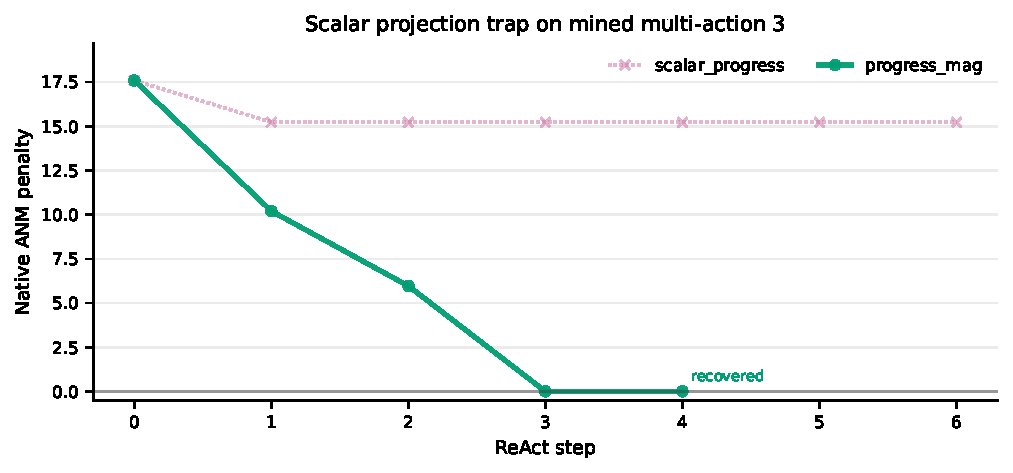
\includegraphics[width=0.44\textwidth]{../figures/mined_multi_action_3_scalar_vs_structured_FINAL.pdf}
\caption{Scalar projection trap on \texttt{multi\_3}. Structured admission (\texttt{progress\_mag}) descends to recovery $\Phi(s){=}(\emptyset,\mathbf{0})$ via accepted \texttt{SAFE\_PROGRESS} steps, whereas the scalar gate admits one early locally-improving proposal and plateaus at nonzero residual across all four slack settings (best $2/7$ at $\eta{=}0.05$).}
\label{fig:trap}
\end{figure}

\subsection{RQ4: Trust-Boundary Containment Under LLM-Side Compromise}
\label{sec:eval:rq4}

The mini-suite runs the three mined multi-action scenarios under \texttt{progress\_mag} with the first three attack families of Sec.~\ref{sec:threat}---prompt injection, observation poisoning, and stall (plain and RAG variants)---at $N{=}5$ per scenario plus a matched benign control: $60$ attack $+\,15$ benign $=75$ episodes, scored by the failure semantics defined there. The fourth family, magnitude redistribution, is evaluated against competing gates below.

Across the $60$ attack episodes the verifier produces $0/60$ attack success, false recovery, and material worsening (Wilson 95\% CI $[0,0.06]$), with $0/15$ on the benign control ($0/75$ overall); under \texttt{prompt\_injection} the rejection rate climbs sharply. Containment is \emph{architectural}, not statistical: the verifier never accesses the LLM's prompt or observation channels (Sec.~\ref{sec:method:shadow}), so any proposal breaching the admission predicates is rejected however the input is corrupted (Prop.~\ref{prop:inv}).

\paragraph{The structured predicate is necessary: magnitude redistribution.}
The fourth family, \emph{magnitude redistribution} (Sec.~\ref{sec:threat}), drives one retained branch toward failure while holding the overloaded-branch set and the aggregate penalty within nominal bounds, evading aggregate- and support-level monitoring. The $39$-episode suite applies this objective across the three scenarios under C1/C2 in three realization variants---direct single-branch concentration, gradual load consolidation, and observation-masked drift (plain and RAG)---all sharing the count-preserving severity signature. A scalar gate is breached $17/39$ and a support-only gate ($\psione\wedge\psitwo$) $12/39$, whereas the full gate ($\psione\wedge\psitwo\wedge\psithree$) is breached $0/39$ (Fig.~\ref{fig:breach}): the aggregate penalty falls and the overloaded-branch \emph{set} is unchanged, so only the per-branch test $\psithree$ rejects the concentrating step.

\begin{figure}[ht]
\centering
\begin{tikzpicture}[font=\sffamily]
  \def\axw{7.2}
  \def\axh{2.7}
  \def\ymax{0.5}
  \pgfmathsetmacro{\sy}{\axh/\ymax}
  \def\bw{1.1}
  \foreach \r in {0,0.1,0.2,0.3,0.4,0.5}{
    \pgfmathsetmacro{\yy}{\r*\sy}
    \draw[gray!22] (0,\yy) -- (\axw,\yy);
    \node[gray!60,font=\scriptsize,left=2pt] at (0,\yy) {\pgfmathprintnumber[fixed,precision=1]{\r}};
  }
  \draw[->,gray!55] (0,0) -- (0,\axh+0.35);
  \draw[gray!55] (0,0) -- (\axw,0);
  \node[gray!70,font=\scriptsize,rotate=90] at (-0.95,\axh/2) {attack breach rate};
  \pgfmathsetmacro{\ha}{0.4359*\sy}
  \fill[oiVermillion] (1.5-\bw/2,0) rectangle (1.5+\bw/2,\ha);
  \node[font=\small\bfseries,above=1pt] at (1.5,\ha) {$17/39$};
  \node[font=\footnotesize,below=3pt] at (1.5,0) {\texttt{scalar}};
  \node[gray!70,font=\scriptsize,below=15pt] at (1.5,0) {aggregate};
  \pgfmathsetmacro{\hb}{0.3077*\sy}
  \fill[oiOrange] (3.6-\bw/2,0) rectangle (3.6+\bw/2,\hb);
  \node[font=\small\bfseries,above=1pt] at (3.6,\hb) {$12/39$};
  \node[font=\footnotesize,below=3pt] at (3.6,0) {\texttt{progress}};
  \node[gray!70,font=\scriptsize,below=15pt] at (3.6,0) {$+$\,support};
  \fill[oiGreen] (5.7-\bw/2,0) rectangle (5.7+\bw/2,0.055);
  \node[font=\small\bfseries,above=2pt,text=oiGreen] at (5.7,0.055) {$0/39$};
  \node[font=\footnotesize,below=3pt] at (5.7,0) {\texttt{progress\_mag}};
  \node[gray!70,font=\scriptsize,below=15pt] at (5.7,0) {$+$\,per-branch};
\end{tikzpicture}
\caption{RQ4: magnitude-redistribution breach rate by admission tier---each added predicate closes more attack surface: scalar $17/39$, support ($\psi_1\wedge\psi_2$) $12/39$, full per-branch ($\psi_1\wedge\psi_2\wedge\psi_3$) $0/39$.}
\label{fig:breach}
\end{figure}

\subsection{RQ5: Generalization Across Families and a Second Domain}
\label{sec:eval:rq5}

The containment result of RQ4 validates the architecture's core invariant; we ask whether the admission-semantics contrast it enables generalizes beyond the primary benchmark.

\paragraph{Cross-family generalization.}
We replicate the terminal-versus-structured contrast across three independent model families---Alibaba Qwen3, Google Gemma-3~\cite{gemma3}, and Meta Llama-3.1~\cite{llama3}---on the same three mined multi-action scenarios at $N{=}5$ (Table~\ref{tab:crossfamily}). The dichotomy is family-independent: terminal deadlocks every model ($0/15$) while structured admission recovers completely ($15/15$ on ANM at $C_{\text{step}}{=}8$), letting compact open-weight models perform the multi-step recovery the terminal gate cannot.

\begin{table}[ht]
\centering
\caption{RQ5: cross-family recovery on the three mined multi-action scenarios, $N{=}5$ (recovery [Wilson 95\% CI]).}
\label{tab:crossfamily}
\footnotesize
\setlength{\tabcolsep}{4pt}
\begin{tabular*}{\textwidth}{@{\extracolsep{\fill}}llccc}
\toprule
Model & Family & terminal & \makecell[c]{\texttt{progress\_mag}\\$C_{\text{step}}{=}8$} & \makecell[c]{\texttt{progress\_mag}\\$C_{\text{step}}{=}16$} \\
\midrule
Qwen3-8B    & Alibaba Qwen3   & $0/15$ & $\mathbf{15/15}$ {\scriptsize[0.80,1.00]} & $15/15$ {\scriptsize[0.80,1.00]} \\
Qwen3-14B   & Alibaba Qwen3   & $0/15$ & $\mathbf{15/15}$ {\scriptsize[0.80,1.00]} & $15/15$ {\scriptsize[0.80,1.00]} \\
Gemma-3-12B & Google Gemma-3  & $0/15$ & $\mathbf{15/15}$ {\scriptsize[0.80,1.00]} & $15/15$ {\scriptsize[0.80,1.00]} \\
Llama-3.1-8B & Meta Llama-3.1 & $0/15$ & $\mathbf{15/15}$ {\scriptsize[0.80,1.00]} & $15/15$ {\scriptsize[0.80,1.00]} \\
\bottomrule
\end{tabular*}
\end{table}

\paragraph{Cross-domain portability.}
We replicate the dichotomy in CityLearn building-energy dispatch~\cite{citylearn} on the same family-spanning subset (Table~\ref{tab:crossdomain}). The three scenarios (\texttt{cl\_1}--\texttt{cl\_3}) instantiate district battery-storage violations (state-of-charge floor/ceiling, feeder-export limits), with $\Phi$ indexed by the violating building or feeder. The gate semantics recur: the terminal predicate clears only the single-step \texttt{cl\_3} ($5/5$) and deadlocks the multi-step \texttt{cl\_1}/\texttt{cl\_2} ($0/10$; the $5/15$ terminal row), while structured admission recovers broadly---$15/15$ for Qwen3-14B and Llama-3.1-8B, $14/15{\to}15/15$ for Qwen3-8B under a doubled budget. Gemma-3-12B reaches $10/15$, its gap confined to \texttt{cl\_2}: the gate admits every Gemma proposal there (all \texttt{SAFE\_PROGRESS}, zero rejections) but its monotone steps stall short of the terminal action stronger models reach. Admission thus ports intact---the gate grades and contains identically---while recovery \emph{completion} remains model-dependent: \emph{structural portability} of the same gate semantics in a distinct physical model.

\begin{table}[ht]
\centering
\caption{RQ5: cross-domain replication on CityLearn (three \texttt{cl} scenarios, $N{=}5$; recovery [Wilson 95\% CI]). \texttt{cl\_3} is single-step recoverable (terminal clears it) while \texttt{cl\_1}/\texttt{cl\_2} are multi-step, mirroring ANM.}
\label{tab:crossdomain}
\footnotesize
\setlength{\tabcolsep}{5pt}
\begin{tabular*}{\textwidth}{@{\extracolsep{\fill}}lccc}
\toprule
Model & terminal & \texttt{progress\_mag} step~$8$ & \texttt{progress\_mag} step~$16$ \\
\midrule
Qwen3-14B    & $5/15$ {\scriptsize[0.15,0.58]}  & $\mathbf{15/15}$ {\scriptsize[0.80,1.00]} & --- \\
Qwen3-8B     & $5/15$ {\scriptsize[0.15,0.58]}  & $14/15$ {\scriptsize[0.70,0.99]} & $\mathbf{15/15}$ {\scriptsize[0.80,1.00]} \\
Gemma-3-12B  & $5/15$ {\scriptsize[0.15,0.58]}  & $10/15$ {\scriptsize[0.42,0.85]} & $10/15$ {\scriptsize[0.42,0.85]} \\
Llama-3.1-8B & $5/15$ {\scriptsize[0.15,0.58]}  & $\mathbf{15/15}$ {\scriptsize[0.80,1.00]} & --- \\
\bottomrule
\end{tabular*}
\end{table}

\subsection{Verifier Overhead}
\label{sec:eval:cost}

Each verifier call performs one $\mathrm{copy}\to\mathrm{apply}\to\mathrm{solve}$ plus three predicate evaluations: $17.5$--$30.0$\,ms on one CPU core, dominated by the solver---under $0.15\%$ of the $\sim$22\,s wall-clock of one LLM ReAct step.

\section{Discussion}
\label{sec:discussion}

\paragraph{Deployment scope.}
\silr{} targets the medium-horizon advisory dispatch loop ($5$--$15$\,min cycles), not the sub-second AGC tick: LLM latency ($\sim$22\,s/step) precludes real-time control, and the shadow-execution model corresponds to the power-flow study preceding every dispatch decision, with protective relays operating independently of the LLM layer.

\paragraph{Support-monotonicity.}
The admission invariant (Prop.~\ref{prop:inv}) assumes recovery needs no transient redistribution: $\psitwo$ forbids steps that overload a new branch, valid in our benchmark. The MPC check (Sec.~\ref{sec:eval:rq3}) recovers the scalar plateau under the same assumption, so the projection trap is gate-induced.

\paragraph{Scope and design properties.}
The security claim is scoped to a \emph{fixed} compromised-LLM adversary on a trusted simulator; adaptive adversaries and simulator--reality mismatch are open.

\paragraph{Future work.}
Two extensions follow: (1)~benchmarks that concurrently activate multiple violation families, where the product order extends across $S$, $\sigma$, and inter-family ordering; (2)~using the graded verdict as a training-time reward, mapping the verdict ladder onto process-reward grading~\cite{lightman2024prm,deepseekmath2024grpo} with a deterministic physics verifier rather than a learned one.

\section{Conclusion}
\label{sec:conclusion}

We studied runtime governance for LLM tool-calling agents under \emph{post-violation recovery admission} and identified the \emph{scalar projection trap}: a scalar gate, as a search operator over the ReAct stream, can commit the trajectory to a residual plateau. We support this with a representational lower bound---no scalar surrogate is sound w.r.t.\ the product order (Prop.~\ref{prop:gap})---an LLM-independent admission invariant (Prop.~\ref{prop:inv}), and an empirical falsifier: scalar slack peaks at $9/21$ (non-monotonic) while structured $\varepsilon$-dominance admission recovers $21/21$ and terminal stalls at $0/21$, the plateau confirmed gate-induced by an MPC check. The dichotomy holds across three model families and reproduces on CityLearn (structural portability), with compact open-weight models recovering the multi-step case; under a fixed compromised-LLM adversary, containment is $0/75$. We will release the scenario library and reference implementation (anonymized for review).


\bibliographystyle{splncs04}
\bibliography{refs}

% Appendix reserved for camera-ready.
%\appendix
%\input{sections/A_appendix}

\end{document}
